%
%  RULES OF THE GAME
%
%  * 80 characters
%  * line breaks at the ends of sentences
%  * eqnarrys ONLY
%  * ``light curve'' not ``light-curve'' or ``lightcurve''
%  * that is all.
%

\documentclass[12pt,preprint]{aastex}

\pdfoutput=1

\usepackage{color,hyperref}
\definecolor{linkcolor}{rgb}{0,0,0.5}
\hypersetup{colorlinks=true,linkcolor=linkcolor,citecolor=linkcolor,
            filecolor=linkcolor,urlcolor=linkcolor}
\usepackage{url}
\usepackage{amssymb,amsmath}
\usepackage{subfigure}

\newcommand{\project}[1]{\textsl{#1}} % hogg say
\newcommand{\kepler}{\project{Kepler}}
\newcommand{\KT}{\project{K2}}
\newcommand{\tess}{\project{TESS}}
\newcommand{\terra}{\project{TERRA}}
\newcommand{\license}{MIT License}
\newcommand{\projectname}{\project{KETU}}

\newcommand{\paper}{\textsl{Article}}

\newcommand{\foreign}[1]{\emph{#1}}
\newcommand{\etal}{\foreign{et\,al.}}
\newcommand{\etc}{\foreign{etc.}}
\newcommand{\True}{\foreign{True}}
\newcommand{\Truth}{\foreign{Truth}}

\newcommand{\figref}[1]{\ref{fig:#1}}
\newcommand{\Fig}[1]{Figure~\figref{#1}}
\newcommand{\fig}[1]{\Fig{#1}}
\newcommand{\figlabel}[1]{\label{fig:#1}}
\newcommand{\Tab}[1]{Table~\ref{tab:#1}}
\newcommand{\tab}[1]{\Tab{#1}}
\newcommand{\tablabel}[1]{\label{tab:#1}}
\newcommand{\Eq}[1]{Equation~(\ref{eq:#1})}
\newcommand{\eq}[1]{\Eq{#1}}
\newcommand{\eqalt}[1]{Equation~\ref{eq:#1}}
\newcommand{\eqlabel}[1]{\label{eq:#1}}
\newcommand{\Sect}[1]{Section~\ref{sect:#1}}
\newcommand{\sect}[1]{\Sect{#1}}
\newcommand{\sectalt}[1]{\ref{sect:#1}}
\newcommand{\App}[1]{Appendix~\ref{sect:#1}}
\newcommand{\app}[1]{\App{#1}}
\newcommand{\sectlabel}[1]{\label{sect:#1}}

\newcommand{\T}{\ensuremath{\mathrm{T}}}
\newcommand{\dd}{\ensuremath{\,\mathrm{d}}}
\newcommand{\bvec}[1]{{\ensuremath{\boldsymbol{#1}}}}
\newcommand{\appropto}{\mathrel{\vcenter{
  \offinterlineskip\halign{\hfil$##$\cr
    \propto\cr\noalign{\kern2pt}\sim\cr\noalign{\kern-2pt}}}}}
\newcommand{\densityunit}{{\ensuremath{\mathrm{nat}^{-2}}}}

% TO DOS
\newcommand{\todo}[3]{{\color{#2} \emph{#1} TODO: #3}}
\newcommand{\dfmtodo}[1]{\todo{DFM}{red}{#1}}
\newcommand{\hoggtodo}[1]{\todo{HOGG}{blue}{#1}}

\begin{document}

\title{%
    \projectname:
    A systematic search for transits in \KT\ data
}

\newcommand{\nyu}{2}
\newcommand{\caltech}{3}
\newcommand{\cfa}{4}
\newcommand{\mpia}{5}
\newcommand{\cds}{6}
\newcommand{\mpis}{7}
\author{%
    Daniel~Foreman-Mackey\altaffilmark{1,\nyu},
    Benjamin~T.~Montet\altaffilmark{\caltech,\cfa},
    David~W.~Hogg\altaffilmark{\nyu,\mpia,\cds},
    Bernhard~Sch\"olkopf\altaffilmark{\mpis},
    Dun~Wang\altaffilmark{\nyu},
    \etal
}
\altaffiltext{1}         {To whom correspondence should be addressed:
                          \url{danfm@nyu.edu}}
\altaffiltext{\nyu}      {Center for Cosmology and Particle Physics,
                          Department of Physics, New York University,
                          4 Washington Place, New York, NY, 10003, USA}
\altaffiltext{\caltech}  {California Institute of Technology, Pasadena, CA,
                          91125, USA}
\altaffiltext{\cfa}      {Harvard-Smithsonian Center for Astrophysics,
                          Cambridge, MA 02138, USA}
\altaffiltext{\mpia}     {Max-Planck-Institut f\"ur Astronomie,
                          K\"onigstuhl 17, D-69117 Heidelberg, Germany}
\altaffiltext{\cds}      {Center for Data Science,
                          New York University,
                          726 Broadway, 7th Floor, New York, NY, 10003, USA}
\altaffiltext{\mpis}     {Max Planck Institute for Intelligent Systems
                          Spemannstrasse 38, 72076 T\"ubingen, Germany}

\begin{abstract}

The photometry from the \KT\ extension of NASA's \kepler\ mission is
afflicted by systematic effects caused by the relative imprecision of the
telescope pointing, and possibly other spacecraft effects.
We present a method for searching these light curves for evidence of
exoplanets by simultaneously fitting for these systematics and the
transit signals of interest.
This method is more computationally expensive than standard search algorithms
but we demonstrate that it can be efficiently implemented and used to
discover transit signals in the existing dataset.
We apply this method to the full Campaign 1 dataset and report a list of XXX
planet candidates transiting YYY stars.
We also present a list of probably astrophysical false positives, and
the results of some follow-up spectroscopic data on a few of the
planet candidates
The most interesting systems are JJJ and HHH.

\end{abstract}

\keywords{%
methods: data analysis
---
methods: statistical
---
catalogs
---
planetary systems
---
stars: statistics
}

\section{Introduction}

The \kepler\ Mission (cite something) has been incredibly succesful at
finding periodic transits (eclipses) in the light curves (time-series
photometry) of stars.
Many of its most important discoveries are long-period planets that
make transits with tiny amplitudes and short durations.
The Mission has demonstrated that it is possible to routinely measure
signals in stellar light curves at the part-in-$10^5$ level, at least
for quiet and apparently bright stars.

At this level of precision, many effects come in to play in a stellar
light curve.
Even in a space observatory like the \kepler\ Satellite, there are
hardware and optics variations that affect simple photometric
measurements at a level greater than part-in-$10^5$.
One of the most serious of these is spacecraft pointing:
If the detector flat-field is not known \emph{exquisitely}, then the
tiny changes to the relative illumination of pixels caused by a star's
motion in the focal plane (or caused by motion of the focal-plane
boresight or orientation relative to the celestial sphere) will lead
to changes in the measured or inferred brightness of the star.
That is, good photometry relies on either a near-perfect flat-field
and pointing model, or else data-analysis techniques that are
insensitive to such variations.
In this \paper\ we present an example of the latter---a
data-analysis technique for exoplanet search and characterization that
is insensitive to spacecraft-induced (or, in general,
hardware-induced) trends in the light curves.

The \KT\ Mission (cite something) is a follow-on to the primary
\kepler\ Mission.
The primary mission came to an end with the failure of a critical
reaction wheel, rendering the spacecraft less able to maintain precise
pointing.
Because of the degraded spacecraft orientation systems, the new
\KT\ data will in general exhibit far greater pointing
variations---and far greater pointing-induced variations in
photometry---than the original \kepler\ data.
This makes good data-analysis techniques all the more valuable.

...simultaneous fitting of systematics and transit signals is a way of
searching for (and measuring) exoplanet signals independent of the
systematics, provided that the systematics lie in the domain of the
model.

...we are not the first to search the \KT\ data (cite Crossfield, etc),
and we build on ideas from \kepler\ searches (cite Petigura and
\kepler).

...The future is \tess (cite something); everything we do here is
highly relevant to that important mission!

\section{Photometry}

The starting point for analysis is the raw pixel data.
We download the full set of XXX target pixel files for \KT's Campaign 1 from
MAST\footnote{\url{https://archive.stsci.edu/k2/}}.
Then, we extract photometry using fixed circular apertures of varying sizes
centered on the mean position of the brightest star (on average) in each
frame.
The centroids and initial flux estimates were measured using
\project{simplexy}, a component of the \project{Astrometry.net} pipeline
\citep{astrometry}.
For each time series, we used 20 circular apertures ranging in radius from 0.5
to 10 pixels and---following \citet{vanderberg-a}---chose the aperture size
that resulted in the smallest CDPP \dfmtodo{CITE CDPP} with a 6 hour
window.\footnote{Note that although we chose a specific aperture, photometry
for every aperture size is available online at \dfmtodo{some URL}.}

Most methods for analyzing \KT\ data---and \kepler\ data, for that
matter---involves some sort of pre-processing or ``de-trending'' step.
For example, \citet{vanderberg-a} measure the centroid motion for each star
and regress out any signal in their aperture photometry that can be fit by
this motion.
Similarly, \citet{crossfield} iteratively construct a robust Gaussian Process
model for the photometry as a function of the measured centroids and de-trend
using the mean prediction from that model.
In our analysis, we don't do any further preprocessing of the light curves
because, as we describe in the next section, we simultaneously fit for the
trends and the transit signals that we are searching for.

One key realization that is also exploited by the official \kepler\ pipeline
is that the systematic trends caused by pointing shifts and other instrumental
effects are shared---with different signs and weights---by all the stars on
the detector.
To exploit this fact, the \project{PDC} component of the \kepler\ pipeline
removes any trends from the light curves that can be fit using a linear
combination of a small number of ``eigen-light curves'' (ELCs) found by
running Principal Component Analysis (PCA) on a set of light curves
\citep{map-pdc1, map-pdc2}.
Similarly, we ran PCA (as implemented by the \project{scikit-learn} project
\citealt{sklearn}) on the full set of Campaign 1 light curves to determine a
basis of representative ELCs.
We chose to use the top 150 components---many more than are normally
used---for our model described in the following section.
\Fig{pca} shows the top few ELCs.


\section{Joint transit \& variability model}

The key insight in our transit search method that sets it apart from the
other standard procedures is that no de-trending is necessary.
Instead, we can fit for the noise (or trends) and signal simultaneously.
This is theoretically appealing because it will be more sensitive to low
signal-to-noise transits.
The main reason for this is that the signal is not exactly orthogonal to the
systematics and the de-trending will over-fit causing the signal to be
distorted and weaker.
In order to reduce this effect, most procedures use a very rigid model for
the trends.
For \KT, this has been implemented by asserting that the centroids contain
all of the information needed to describe the trends.
In the \kepler\ pipeline, this is implemented by only allowing a small number
of PCA components to contribute to the fit.

Physically, the motivation for our model---and the PDC model---is that every
star on the detector should be affected by same set of systematic effects.
These are caused by things like pointing jitter, temperature variations, and
other sources of PSF modulation and each one will be imprinted in the light
curves of many stars with varying amplitudes and signs.
Therefore, while it is hard to write down a physical generative model for the
systematics, building a data-driven model might be possible.
This intuition is also exploited by other methods that model the systematics
using only empirical centroids \citep{vanderberg-a, crossfield} but out more
flexible model should capture the systematic effects more robustly but there
is a risk of over-fitting.
\Fig{corr} shows the application of this model to a light curve with no known
transit signals.

To avoid over-fitting in our pipeline, we simultaneously fit for the transit
signal and the trends using a rigid model for the signal and a relatively
flexible model for the noise.
Specifically, we model the light curve as being generated by linear
combination of the 150 basis light curves and a ``box'' transit model at a
given period and phase.


\section{Search pipeline}

In theory, search could proceed by evaluating the model described above on a
fine grid three-dimensional grid in period, phase, and duration.
In practice, this is computationally intractable for any grids of the
required size.
Instead, we can compute the values on this grid approximately, but at very
high precision, using a two-step procedure that is much more computationally
efficient.
The first step, called the {\bf linear search}, involves hypothesizing a
single transit on a two-dimensional grid in duration and transit time.
The second step, the {\bf periodic search} uses a lookup table built on the
results of the linear search to compute the likelihood for the periodic model.
Finally, the peaks in the likelihood space are passed along for machine and
hand vetting.

\paragraph{Linear search}

The linear search involves hypothesizing a transit signal on a
two-dimensional grid in transit time and duration.
For each point in the grid, we use the model described in the previous
section to evaluate \emph{the likelihood function} of the transit depth.
Because the model is linear, the likelihood function for the depth
(marginalized over the model of the systematics) is a Gaussian:
\begin{eqnarray}
\ln \mathcal{L} (d) &\propto& \mathcal{N} ()
\end{eqnarray}

\paragraph{Periodic search}

\paragraph{Machine vetting}

\paragraph{Hand vetting}


\section{Results}

\section{Discussion}

\acknowledgments
It is a pleasure to thank
\ldots\
for helpful contributions to the ideas and code presented here.
This project was partially supported by the NSF (grant AST-0908357), NASA
(grant NNX08AJ48G), and the Moore--Sloan Data Science Environment at NYU.
This research made use of the NASA \project{Astrophysics Data System}.

\newcommand{\arxiv}[1]{\href{http://arxiv.org/abs/#1}{arXiv:#1}}
\begin{thebibliography}{}\raggedright

\bibitem[Crossfield \etal(2015)]{crossfield}
Crossfield, I.~J.~M., Petigura, E., Schlieder, J., \etal\ 2015,
\arxiv{1501.03798}

\bibitem[Lang \etal(2010)]{astrometry}
Lang, D., Hogg, D.~W., Mierle, K., Blanton, M., \& Roweis, S.\ 2010, \aj, 139,
1782

\bibitem[Pedregosa \etal(2011)]{sklearn}
Pedregosa, F., Varoquaux, G., Gramfort, A., \etal\ 2011, JMLR, 12, 2825

\bibitem[Smith \etal(2012)]{map-pdc2}
Smith,~J.~C., Stumpe,~M.~C., Van Cleve,~J.~E., \etal\ 2012,
\pasp, 124, 1000

\bibitem[Stumpe \etal(2012)]{map-pdc1}
Stumpe,~M.~C., Smith,~J.~C., Van Cleve,~J.~E., \etal\ 2012,
\pasp, 124, 985

\bibitem[Vanderburg \& Johnson(2014a)]{vanderberg-a}
Vanderburg, A., \& Johnson, J.~A.\ 2014, \pasp, 126, 948

\bibitem[Vanderburg \etal(2014b)]{vanderburg-b}
Vanderburg, A., Montet, B.~T., Johnson, J.~A., \etal\ 2014, \arxiv{1412.5674}

\end{thebibliography}

\clearpage
\appendix

\section{Mathematical model}\sectlabel{math}

Formally, this can be written for the light curve of the $k$-th star as
\begin{eqnarray}\eqlabel{linear-model}
\bvec{f}_k &=& \bvec{A}\,\bvec{w}_k + \mathrm{noise}
\end{eqnarray}
where
\begin{eqnarray}
\bvec{f}_k &=& \left (\begin{array}{cccc}
    f_{k,1} & f_{k,2} & \cdots & f_{k,N}
\end{array}\right )^\T
\end{eqnarray}
is the list aperture fluxes for star $k$ observed at $N$ times
\begin{eqnarray}
\bvec{t} &=& \left (\begin{array}{cccc}
    t_{1} & t_{2} & \cdots & t_{N}
\end{array}\right )^\T \quad.
\end{eqnarray}
In \eq{linear-model}, the design matrix is given by
\begin{eqnarray}
\bvec{A} &=& \left (\begin{array}{cccccc}
    x_{1,1} & x_{2,1} & \cdots & x_{J,1} & 1 & m_\bvec{\theta}(t_1) \\
    x_{1,2} & x_{2,2} & \cdots & x_{J,2} & 1 & m_\bvec{\theta}(t_2) \\
    && \vdots &&&\\
    x_{1,N} & x_{2,N} & \cdots & x_{J,N} & 1 & m_\bvec{\theta}(t_N)
\end{array}\right )
\end{eqnarray}
where the $x_{j,n}$ are the basis ELCs---with the index $j$ running over
components and the index $n$ running over time---and $m_\bvec{\theta}(t)$ is
the transit model
\begin{eqnarray}
m_\bvec{\theta}(t) &=& \left\{\begin{array}{cl}
-1 & \mathrm{if\,}t\,\mathrm{in\,transit} \\
0 & \mathrm{otherwise}
\end{array}\right.
\end{eqnarray}
parameterized by a period, phase, and transit duration (these parameters are
denoted by \bvec{\theta}).

Assuming that the uncertainties on $\bvec{f}_k$ are Gaussian and constant,
the maximum likelihood solution for \bvec{w} is
\begin{eqnarray}
{\bvec{w}_k}^* &\gets& \left( \bvec{A}^\T\,\bvec{A} \right)^{-1}\,
                       \bvec{A}^\T\,\bvec{f}_k
\end{eqnarray}
and the marginalized likelihood function for the transit depth is a Gaussian
with the mean given by the last element of ${\bvec{w}_k}^*$ and the variance
given by the lower-right element of the matrix
\begin{eqnarray}
{\bvec{\delta w}_k}^2 &\gets& {\sigma_k}^2 \,
            \left( \bvec{A}^\T\,\bvec{A} \right)^{-1}
\end{eqnarray}
where $\sigma_k$ is the uncertainty on $\bvec{f}_k$.
The amplitude of this Gaussian is given by
\begin{eqnarray}\eqlabel{depth-likelihood}
\mathcal{L}_k &=& \frac{1}{(2\,\pi\,{\sigma_k}^2)^{N/2}}\,\exp\left(
-\frac{1}{2\,{\sigma_k}^2}\,
\left| \bvec{f}_k - \bvec{A}\,{\bvec{w}_k}^* \right|^2
\right)
\end{eqnarray}
evaluated at the maximum likelihood value ${\bvec{w}_k}^*$.

Remember that the likelihood defined in \eq{depth-likelihood} is a function of
the parameters \bvec{\theta} (the period, phase, and duration of the planet).
In principle, this means that a transit search can proceed by building a dense
3D grid of \bvec{\theta} values and evaluating the likelihood of the data
$\mathcal{L}_k$ using \eq{depth-likelihood} at each point in the grid.

\clearpage

\begin{figure}[p]
\begin{center}
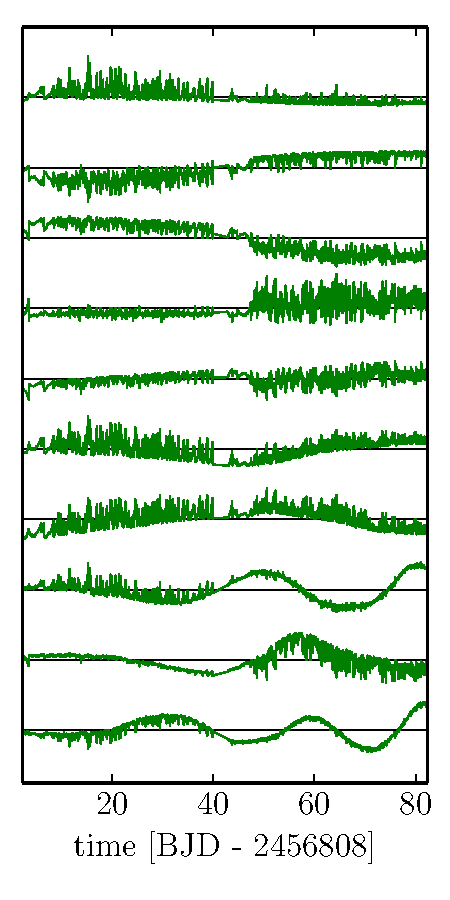
\includegraphics{figures/pca.pdf}
\end{center}
\caption{%
A CAPTION.
\figlabel{pca}}
\end{figure}

\begin{figure}[p]
\begin{center}
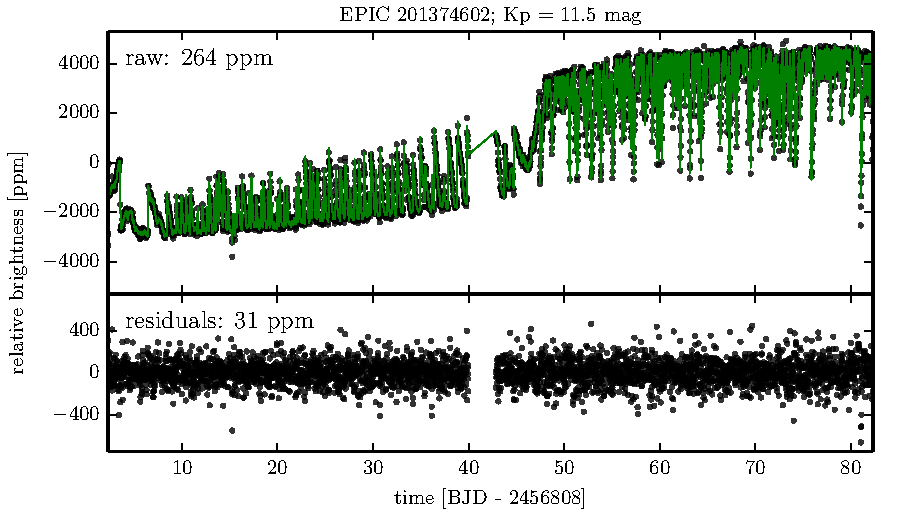
\includegraphics{figures/corr.pdf}
\end{center}
\caption{%
A CAPTION.
\figlabel{corr}}
\end{figure}

\end{document}
